\documentclass[titlepage]{article}

\usepackage{float}
\usepackage[T1]{fontenc}
\usepackage[utf8]{inputenc}
\usepackage[english]{babel}
\usepackage{minted}
\usepackage{graphicx}
\usepackage{geometry}
\usepackage{amsmath}
\usepackage{appendix}
\usepackage{comment}
\usepackage{hyperref}
\usepackage{caption}
\usepackage{amssymb}

\usepackage{fancyvrb}
\usepackage{csquotes}

\usepackage{xcolor}
\usepackage{listings}
\usepackage{enumitem}
\usepackage{amsfonts}
\usepackage{array,booktabs,makecell,multirow}
\usepackage{siunitx}

\geometry{hmargin=3cm,vmargin=2cm}

\usepackage[
backend=biber,
style=alphabetic,
sorting=ynt
]{biblatex}
\addbibresource{ref.bib}

\begin{document}
\begin{titlepage}
\newcommand{\HRule}{\rule{\linewidth}{0.5mm}}
\center
\textsc{\LARGE
Information and Coding Theory 
} \\[1cm]
\textsc{\LARGE
ELEN060-2
} \\[1cm]

\includegraphics[scale=0.2]{logo.jpg} \\[3cm]
\HRule \\[0.4cm]
{ \huge \bfseries Project 2 - Source coding, data compression and channel coding \\[0.15cm] }
\HRule \\[1.5cm]
Destexhe Clara S191103 \\
Hogge Louis S192814
\\[1.5cm]
\today \\ [1cm]
\end{titlepage}

\section{Implementation}
\subsection{Question 1 : }

The main steps of the implementation are:
\begin{enumerate}
    \item Find the indices of the two nodes with the smallest probabilities.
    \item Build the Huffman tree based on the given probability distribution.
    \item Recursively generate Huffman codes from the Huffman tree.
\end{enumerate}
For the given example, the output of the implementation is:

\begin{table}[h!]
    \centering
    \small
    \setlength{\tabcolsep}{4pt}
    \begin{tabular}{|p{2cm}|p{2cm}|}
        \hline 
        \textbf{Symbol} & \textbf{Codeword}  \\
        \hline
        \textit{S1} & '000'\\
        \hline
        \textit{S2} & '001'\\
        \hline
        \textit{S3} & '100'\\
        \hline
        \textit{S4} & '101'\\
        \hline
        \textit{S5} & '01'\\
        \hline
        \textit{S6} & '11'\\
        \hline
    \end{tabular}
    \caption{Output}
    \label{tab:q1}
\end{table}
Which is not identical to the solution provided in TP2 but when there are various options for merging two nodes with the lowest probabilities, we know that there are multiple optimal Huffman codes. The one provided here can be verified by hand.\\

To extend the function to generate a Huffman code of any (output) alphabet size, the Huffman coding algorithm must be altered such that it generates a multiway tree rather than a binary tree. Here is a rough overview:
\begin{itemize}
    \item[-] \textit{Initialization:} Create a node for each distinct tuple of n symbols, where n is the number of symbols in your alphabet, as opposed to making one for each symbol and giving it a frequency. Set the frequency of each node to match the frequency of the input tuple.
    \item[-] \textit{Building the tree:} Join the n nodes with the smallest frequency as opposed to always merging the two nodes with the smallest frequency. These n nodes are created as children of a new node with a frequency equal to the sum of their individual frequencies.
    \item[-] \textit{Assigning codes:} Instead of giving one branch a 0 and the other a 1, give each branch a distinct symbol from your alphabet.
    \item[-] \textit{Encoding:} Replace each tuple of n symbols in a string with its appropriate code.
    \item[-] \textit{Decoding:} To decode a string, replace each code with the tuple of n symbols that it corresponds with.
\end{itemize}

\newpage

\subsection{Question 2 : }

For the given example, the output of the implementation is:

\begin{table}[h!]
    \centering
    \small
    \setlength{\tabcolsep}{4pt}
    \begin{tabular}{|p{3.5cm}|p{3cm}|p{3cm}|}
        \hline
        \multicolumn{1}{|p{3.5cm}|}{\textbf{Symbol}} & \multicolumn{2}{p{6cm}|}{\textbf{Codeword}}\\
        \cline{2-3} 
         & entry index & binarized adress with one appended symbol \\
        \hline
        ' ' & 0 & ' ' \\
        \hline
        '1' & 1 & '1' \\
        \hline
        '0' & 2 & '00' \\
        \hline
        '11' & 3 & '011' \\
        \hline
        '01' & 4 & '101' \\
        \hline
        '010' & 5 & '1000' \\
        \hline
        '00' & 6 & '0100' \\
        \hline
        '10' & 7 & '0010' \\
        \hline
        \multicolumn{1}{|p{3.5cm}|}{\textbf{Encoded sequence}} & \multicolumn{2}{p{6cm}|}{100011101100001000010} \\
        \hline
    \end{tabular}
    \caption{Output}
    \label{tab:q2}
\end{table}
Which is coherent with the solution given in the theoretical course.

\subsection{Question 3 : }

\textbf{Basic Lempel-Ziv Algorithm:}
\begin{itemize}
    \item[$\bullet$] \textit{Advantages:}
    \begin{itemize}
        \item[-] It is a universal algorithm, able to asymptotically approach the entropy of any stationary ergodic source.
    \end{itemize}
    \item[$\bullet$] \textit{Drawbacks:}
    \begin{itemize}
        \item[-] Source must be stationary and ergodic.
        \item[-] Address coding: it predefines the binary address length, potentially wasting space for small input text or proving insufficient for large ones.
    \end{itemize}
\end{itemize}
\textbf{On-line Lempel-Ziv Algorithm:}
\begin{itemize}
    \item[$\bullet$] \textit{Advantages:}
    \begin{itemize}
        \item[-] It adapts the address length based on the current dictionary size allowing it to better handle changes in the data distribution.
        \item[-] It is robust and makes no assumptions about the source behavior.
    \end{itemize}
    \item[$\bullet$] \textit{Drawbacks:}
    \begin{itemize}
        \item[-] The asympotic performances are reached only when the dictionary starts to become representative, i.e., it contains a significant fraction of sufficiently long typical messages. So for very long texts.
        \item[-] Not very competitive in general due to robustness.
    \end{itemize}
\end{itemize}

\subsection{Question 4 : }

For the given example, the output of the implementation is:

\begin{table}[h!]
    \centering
    \small
    \setlength{\tabcolsep}{4pt}
    \begin{tabular}{|p{3.5cm}|p{3.5cm}|}
        \hline 
        \textbf{Encoded sequence} & 00a00b00r31c21d74d  \\
        \hline
    \end{tabular}
    \caption{Output}
    \label{tab:q4}
\end{table}
Which is coherent with the solution given in the theoretical course.

\section{Source coding and reversible data compression}
\subsection{Question 5 : Image display}

One image has been provided in two different formats, the first one has been encoded with pixel values, each pixel is assigned to a brightness value between 0 and 255 encoded in byte. The second one has been encoded in PNG format in hexadecimal. \\

To read and display the first image, a \textit{display$\_$image} function has been implemented taking in input the path to access the image. First, the function convert hexadecimal numbers in integers. Then, it creates a new image of dimensions 512x512, and put each pixel at its place. \\

To read and display the second image, a \textit{display$\_$image$\_$png} has been implemented taking in put the path to access the image. First, the function reads the file and then converts hexadecimal numbers in bytes. Finally, it displays the image. \\

As said before, the dimensions of the images are 512x512 meaning the image contains 262 144 pixels. For the first image, each pixel is assigned to a brightness value between 0 and 255. Therefore, the number of symbols required is :

$$ n_{symb} = 256^{n_{pixels}} = 1,3 * 10^{198 657} $$ For the second image, as PNG is a format for which any image can be represented. It is due to the fact png is a lossless compression format meaning any image can be recovered from its compressed version. 

Concerning the length of the files, for the raw grayscale image pixel format, each pixel is encoded thanks to only one byte. Therefore, the length of this format can be computed as :

$$l1 = 512*512 = 262\text{ } 144 \text{ bytes}$$ 

However, for the PNG format, each pixel is represented by several bytes. The length of the PNG file is the number of column multiplied by the number of lines of the PNG.txt file. 

$$l2 = 8 * 20 \text{ } 069 = 160\text{ }552 \text{ bytes} $$
 
\subsection{Question 6 : Binary Huffman code for PNG file }

To compute the marginal probability of all symbols, we need to count the number of occurrence of each symbol and then divide it by the total number of symbols. The total number of symbols is equal to the number of columns multiplied by the number of lines of the png.txt file. Therefore, total$\_$nb = 8 * 20 069 = 160 552.
$$ P(S_i) = \frac{\#S_i}{\sum^\text{160 552}_{i=1}\#S_i}$$ for i = 1,...,160 552.

Then, this marginal probability distribution is given in input to the \textit{Huffman$\_$code()} function. This gives the Huffman code for each symbol (the Huffman code can be found in the jupyter notebook). Each number is represented by 8 bits in the PNG file. The total length of the encoded PNG sequence is then the number of bits for each pair of hexadecimal number multiplied by the total number of pair (computed in the jupyter notebook). Therefore, 
$$ \text{Length encoded PNG sequence} = 1 \text{ } 282 \text{ } 749 \text{ bits}$$
$$ \text{Length PNG sequence} = 8 * 160 552 = 1 \text{ } 284 \text{ } 416 \text{ bits}$$
The compression rate can be computed as : 

$$ \text{Compression rate} = \frac{\text{length PNG}}{\text{length encoded PNG}} = 1,0013$$

\subsection{Question 7 : Huffman code expected average length}
The Huffman code expected average length can be computed with the formula : 

$$\bar{n}=\sum_{i=1}^R P\left(S_i\right) \cdot n_i= 7,989617 \text{ bits}$$

where R is the number of different symbols, $P(S_i)$ the probability of each symbol and $n_i$ the length of the Huffman code for the considered symbol. In other words, in average, the Huffman length code for each symbol is equal to about 8 bits. \\

The empirical average length is also equal to 7,989617 as we compute the Huffman code with empirical probabilities calculated on the same image as the one used to build the code. The theoretical bounds is written as : 
$$ \frac{H(S)}{log_2 q} \leq \bar{n} < \frac{H(S)}{log_2 q} + 1$$
The entropy is computed thanks to a function \textit{Entropy()}, 
$$H(S) = 7.9722$$
Therefore, 
$$ 7.972 \leq \bar{n} < 8.972$$
The expected average length is included in the bounds. The code is optimal as stated by the first Shanon theorem. Therefore,  this algorithm provides an optimal and prefix-free code. 

\subsection{Question 8 : Empirical average length plot}

The figure \ref{fig:Q8} represents the evolution of the empirical average length for different values of file length. It can be observed that the empirical average length is increasing with the file length. It can be explained as shorter the file, shorter is the Huffman code of the symbols. Indeed, in shorter files, the symbols are more present, therefore, their probability distribution will be higher. This evolution has a limit as we reach a plateau for larger value of file lengths. Indeed, the probability distribution of all symbols tends to their real values. The empirical average length converges to the expected average length.  
\begin{figure}[H]
  \centering
  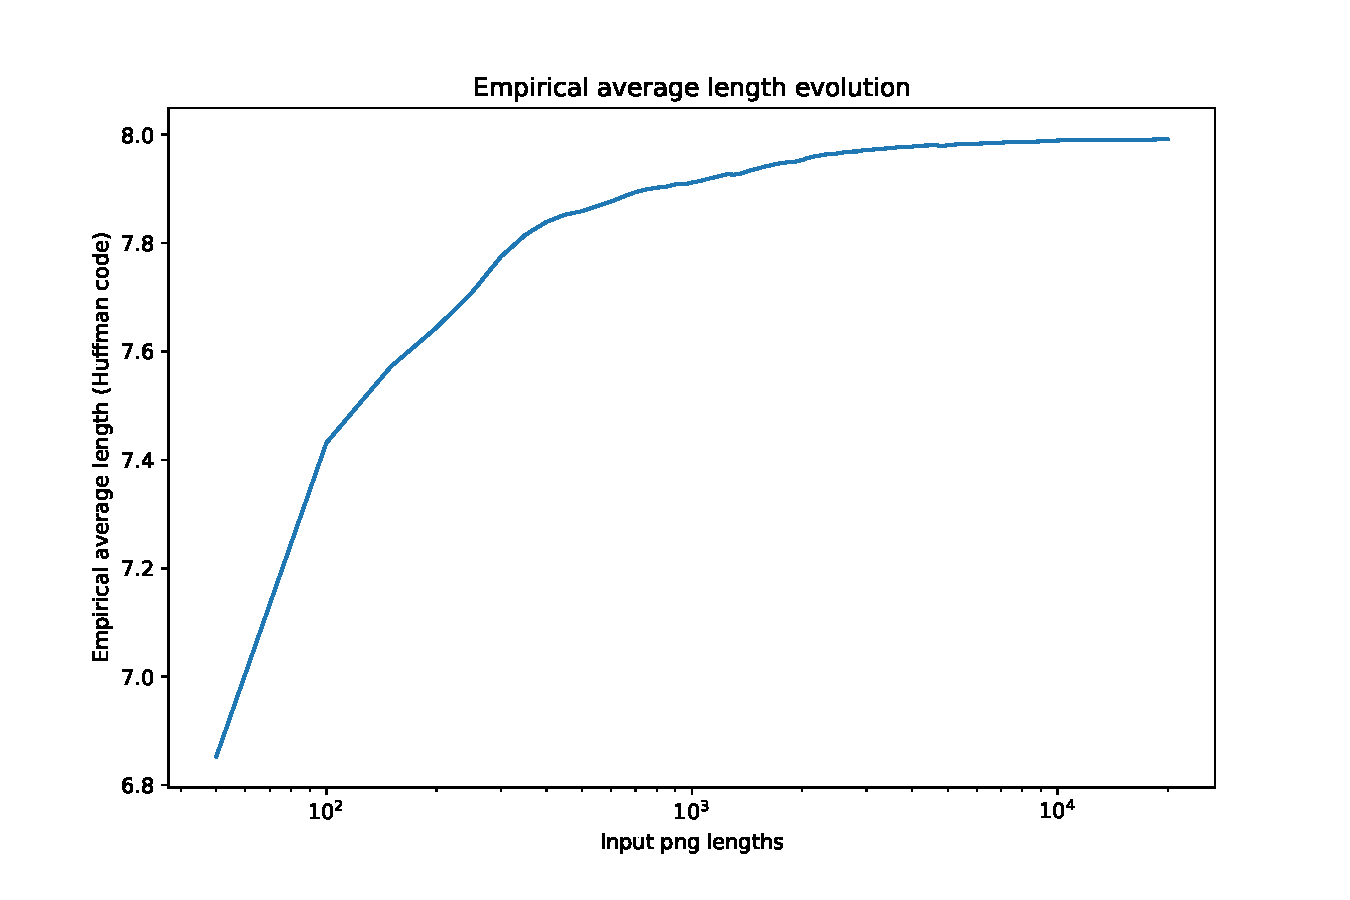
\includegraphics[scale=0.4]{Q8.pdf}
  \caption{Empirical average length evolution of the Huffman code as file length function }
  \label{fig:Q8}
\end{figure}

\subsection{Question 9 : On-line Lempel-Ziv algorithm}

In order to apply the algorithm on the PNG file, we needed to adapt the function \textit{LZ$\_$online}. We created a function \textit{LZ$\_$online$\_$hexa} that gives a dictionary for keys as hexadecimal numbers. We needed also to "pre-process" to split the file in pair of hexadecimal numbers. After that, we apply the algorithm on the PNG file, the new function gives in output the dictionary and the encoded sequence for the specific PNG file. \\

The length of the encoded sequence in bits is equal to 1 540 629 bits. The compression rate can be computed as : 
$$ \text{Compression rate } = \frac{\text{PNG file length}}{\text{Encoded PNG file length}} = 0,833696$$

This result is not sufficient as the length of the compressed file is larger than the original file.

\subsection{Question 10 : LZ77 algorithm with window$\_$size=7}

In order to apply the algorithm on the PNG file, we needed to adapt the function \textit{LZ77}. We created a function \textit{LZ$\_$hexa} that gives a dictionary for keys as hexadecimal numbers. We needed also to "pre-process" to split the file in pair of hexadecimal numbers. After that, we apply the algorithm on the PNG file, the new function gives in output the encoded sequence for the specific PNG file. \\

The length of the encoded sequence in bits is equal to 2 480 432 bits. 
The compression rate can be computed as : 
$$ \text{Compression rate } = \frac{\text{PNG file length}}{\text{Encoded PNG file length}} = 0,517819$$
This technique is not really efficient. 

\subsection{Question 11 : Combination of the two algorithms} 

As a reminder, the LZ77 and the Huffman algorithm are lossless compression algorithms. One way to combine these algorithms is the LZ77-Huffman compression. First, this combined algorithm performs LZ77 compression to generate an intermediate compressed buffer which finds repeated patterns in the data and replace them with references to earlier occurrences of those patterns. Secondly, the resulting data is compressed with the Huffman algorithm. This way to operate is effective as LZ77 finds first patterns in the data and then this resulting data is likely to have many repeated symbols, which can be more efficiently encoded using Huffman coding. \\

A second way to combine these two compression algorithms is the LZHUF compression. The principle is to use Huffman coding to encode the dictionary used by the LZ77 algorithm. Huffman coding makes the resulting codes more compact. It helps with compression gains, especially if the dictionary is large of contains many infrequent symbols.  \\

In conclusion, the combination of these two algorithms improves the compression. Each algorithm has its own forces and combined, the compression is more effective. Indeed, the LZ77 is effective at finding repeated patterns and Huffman is good at compressing individual symbols. 


\subsection{Question 12 : Code of the combination}

To combine the two algorithms, we decided to code the first method. The result of the LZ77-Huffman algorithm is a mix of number symbols and binary number from the Huffman code. The resulting length is : 
$$\text{Length of the PNG encoded} = \text{3 696 200 bits}$$
The length is higher as it takes into the account the symbols of the LZ77 and the Huffman algorithm. 
$$\text{Compression rate = 0,694993}$$

The result is not very sufficient as the encoded pixel file is longer than the initial file. 

\subsection{Question 13 : Comparison }

The figures \ref{fig:Q13_c} and \ref{fig:Q13_l} make a comparison between the LZ77 algorithm and LZ77-Huffman algorithm. For the LZ77 algoritm, the compression rate is stable. It only decreases a little for small window sizes. For the LZ77-Huffman algorithm, a big increase happens for small window sizes and then the increase is stabilized. We can also see that for the length of the encoded sequence, it is stable for LZ77. At the level of the LZ77-Huffman algorithm, first, it increases sharply and then stabilizes. The larger the window, the larger the number of previously encoded symbols can be referenced, which can lead to more efficient compression\\

The compression rate is better for the LZ77-Huffman algorithm, which is logical as the LZ77-Huffman is more efficient than the LZ77 one. If we compare the compression rates, the more efficient is the LZ77-Huffman, then the LZ-online and finally the LZ77. LZ-Huffman needs larger window to work efficiently.  The LZ-online and the LZ77 provide low quality compression as the compression rates are below one. Therefore, the encoded sequence are longer than the initial file. 

\begin{figure}[h!]
    \begin{minipage}[c]{0.5\linewidth}
        \centering
        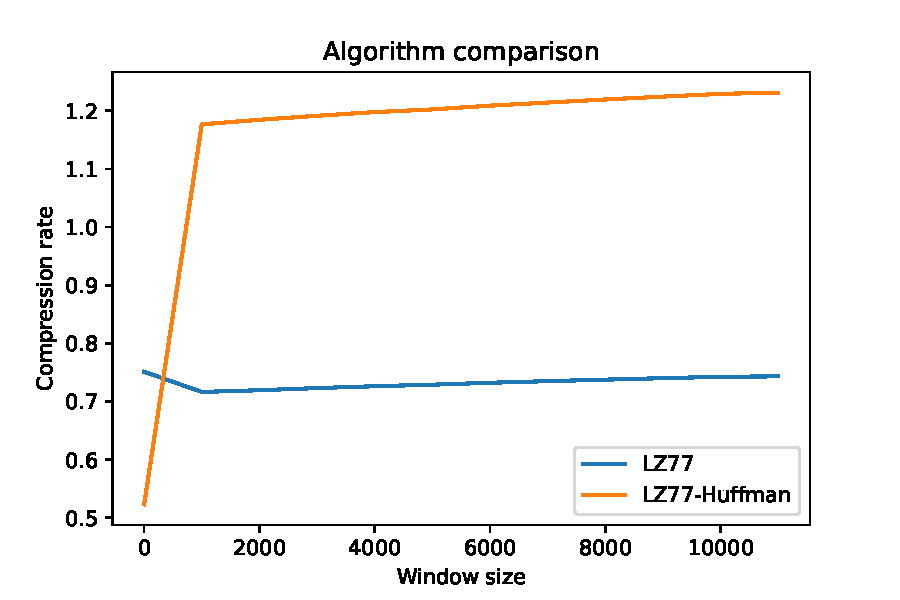
\includegraphics[scale = 0.5]{Q13_c.pdf}
        \caption{Compression rate comparison}
        \label{fig:Q13_c}
    \end{minipage}
    \hfill%
    \begin{minipage}[c]{0.5\linewidth}
        \centering
        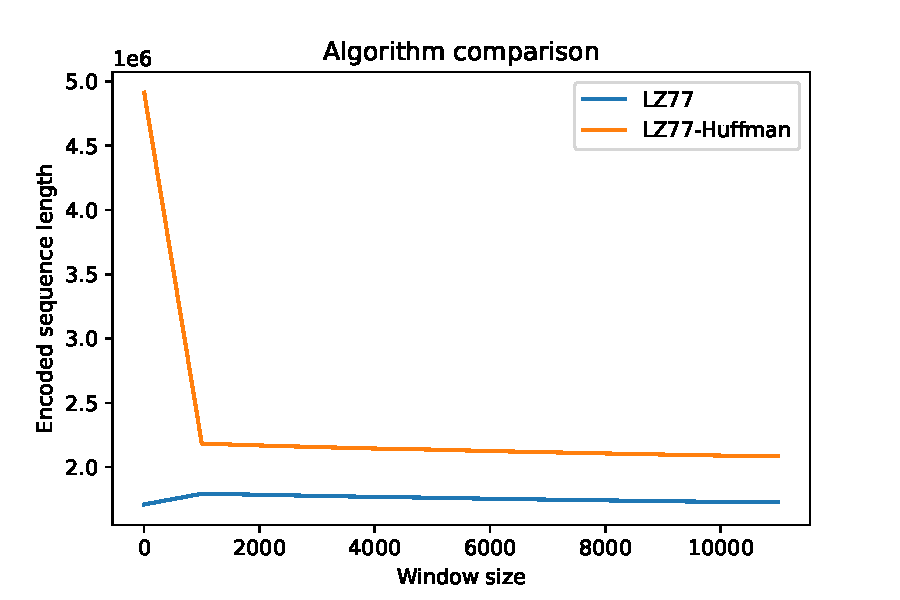
\includegraphics[scale = 0.5]{Q13_l.pdf}
        \caption{Encoded sequence length comparison}
        \label{fig:Q13_l}
    \end{minipage}
\end{figure}


\subsection{Question 14 : Huffman code for pixel file}
This question is the same as question 5 but by doing it for the "pixel.txt" file. To compute the marginal probability of all symbols, we need to count the number of occurrence of each symbol and then divide it by the total number of symbols. The total number of symbols is has been determined before and is equal to 262 144 bytes. 
$$ P(S_i) = \frac{\#S_i}{\sum^\text{262 144}_{i=1}\#S_i}$$ for i = 1,...,262 144.

Then, this marginal probability distribution is given in input to the \textit{Huffman$\_$code()} function. This gives the Huffman code for each symbol (the Huffman code can be found in the jupyter notebook). The total length of the pixel file can be computed as : 
$$ \text{Length pixel sequence} = 8 * 262 144= 2 \text{ } 097 \text{ } 152 \text{ bits}$$
$$ \text{Length encoded pixel sequence} =  1\text{ } 584 \text{ } 881 \text{ bits}$$ 
The compression rate can be computed as : 

$$ \text{Compression rate} = \frac{\text{length pixel}}{\text{length encoded pixel}} = 1,328271$$ 
The compression rate is a little above one, which is satisfying for a compression. The averaged length can be computed with the formula : 

$$\bar{n}=\sum_{i=1}^R P\left(S_i\right) \cdot n_i= 6,04584 \text{ bits}$$

where R is the number of different symbols, $P(S_i)$ the probability of each symbol and $n_i$ the length of the Huffman code for the considered symbol. In other words, in average, the Huffman length code for each symbol is equal to about 6 bits.  The empirical average length is the same and is equal to 6,04584 bits. \\

\subsection{Question 15 : Comparison}

If we encode directly the pixel file with Huffman, we obtain a better compression rate (1,026997) in comparison to compressing the PNG file (1,0013). It is due to the fact the PNG is already a coded image. 
Moreover, the length of the pixel encoded file is lower than the PNG encoded sequence. We observe that using directly the pixel file yields better results. It is due to the fact encoding an image two times (PNG file) is less efficient than only encode one time the image (pixel file). In other words, Huffman coding is less effective on data where there are very few unique symbols, or where the symbols are already highly compressed (PNG file). \\

In conclusion, we will prefer using the pixel values directly than using a pre-compressed file. 

\section{Channel coding}

\subsection{Question 16 : }

The original text:

\begin{displayquote}
    THE BOY WHO LIVED Mr. and Mrs. Dursley, of number four, Privet Drive, were proud to say that they were perfectly normal, thank you very much. They were the last people you'd expect to be involved in anything strange or mysterious, because they just didn't hold with such nonsense. Mr. Dursley was the director of a firm called Grunnings, which made drills. He was a big, beefy man with hardly any neck, although he did have a very large mustache. Mrs. Dursley was thin and blonde and had nearly twice the usual amount of neck, which came in very useful as she spent so much of her time craning over garden fences, spying on the neighbors. The Dursley s had a small son called Dudley and in their opinion there was no finer boy anywhere. The Dursleys had everything they wanted, but they also had a secret, and their greatest fear was that somebody would discover it. They didn't think they could bear it if anyone found out about the Potters. Mrs. Potter was Mrs. Dursley's sister, but they hadn't met for several years; in fact, Mrs. Dursley pretended she didn't have a sister, because her sister and her good-for-nothing husband were as unDursleyish as it was possible to be. The Dursleys shuddered to think what the neighbors would say if the Potters arrived in the street. The Dursleys knew that the Potters had a small son, too, but they had never even seen him. This boy was another good reason for keeping the Potters away; they didn't want Dudley mixing with a child like that. When Mr. and Mrs. Dursley woke up on the dull, gray Tuesday our story starts, there was nothing about the cloudy sky outside to suggest that strange and mysterious things would soon be happening all over the country. Mr. Dursley hummed as he picked out his most boring tie for work, and Mrs. Dursley gossiped away happily as she wrestled a screaming Dudley into his high chair. None of them noticed a large, tawny owl flutter past the window. At half past eight, Mr. Dursley picked up his briefcase, pecked Mrs. Dursley on the cheek, and tried to kiss Dudley good-bye but missed, because Dudley was now having a tantrum and throwing his cereal at the walls. "Little tyke," chortled Mr. Dursley as he left the house. He got into his car and backed out of number four's drive.
\end{displayquote}

The number of bits required to encode the text signal of the text provided with this assignment, using the binary ASCII fixed-length binary code, is 18088 bits.

\subsection{Question 17 : }

The decoded text contains errors due to the noise introduced by the channel effect: 

\begin{displayquote}
    TIE BOY`WHO LIVAE Mr. and Mrs. Dusslåy¬(nf nueber four,0Privet Drkve, w\%ru prout)tg sey that tjey weòe pgrfectly noríal, thank you veri much. Thg9 were txe¤last peoxle you¯d expect to je iovolree in anythinf stra.wg or mysterio5r, becqusm Thei ju3t° didn't hml\$ with sucj nonqensen(Mr. DurSley was The director(of a firm called Grõnniogs, wh)ch eaee dri,|w. He was a big, beefy man with habd|y any neck, altho5gh he0did have a fery larue mustache. Mrs. DuRsle\{ wAs(vxin anä âlonde and had neerly tw)ce uhe useal ammuNt of nu\#k, Which came i very usefuL as sh spunt so muCh gf éer time craîing over garden fences, spyinc on the .eighboss. The Dur\{ley s had a cmall son callmd DuDley and0in their opiniïn there was¨nï finer boy anyw(ere. The Dursleys h`d everything they wajted,but they alsg had c secrut, a~d their wreaô\%st Fear waó that soieboäy g/uld discover it. Thay d)dn't thinkthdy cnUld b\%ar it if anyone found out abouT the Pottdrs. Mrs. Pïtter was Mbs. Fursley'q sister, but tèey hafn't meT foò seVòal years;0in fAãt( Mrs.!Dursley`@2etended she dIdn'p havm a 3istEr, becatse her qisdeR and hur go/d-for-ootèine hu3band vere as!unDuÒsleyishpa\{ iô was powsible t bd> The Dtrslmys shudfered to txi.k(what tbe neighbors wmuld@sáy if the0Pott\%ró arrivud i~ thg stremt\& The Dõrsheys \{new tèat the Potterc haf a s-all(son, too, `ut they h!\$ never even seen him. This boy was another good reaso~ for keeping*the Pktters away; thEy didn't want Dudley mixinc with c child like that.!W`en Mr. aîd Íòs. DursleY \}oie wp on0the dell, gRay Ôuesday our`s|ory stabts, there!wis nothing about phe"cloudY sky outside to seggeRt that stòanGe and mysteriou\{ t`infs wlu,` skonre iappenino all oVer the count2y. Mr. D5òsleyhulmed as he pickgd out hi\{ eost borinG tie for work,"aîd Lrsn Dursley!gossipedawa9 hqPpily as sh\% wrestlef"a\$scrdaming"Dudleyanto his hieè chais. None /f thEm notkced a larGe, tawjy owl flutter p!st`the 7intow. At laLf past0eIghv, Mr. Dõrsley pickåd up his briefc`se, peckef ]ss. DUròle\}on ôhe cheek- and tried to\$cIss Duäley good-bye but`miSsed,(because Dudley was now having a tantrUm and thrïwing hhs cepeel at the walhs. "L)ttle tykE," chorulgd Mr. Dursley as he left\$the iousm. Hm got iîto his cir"aîd backed\$oet on nember`fo5r's Drive. 
\end{displayquote}

\subsection{Question 18 : } 

See jupyter notebook 

\subsection{Question 19 : }

The decoded text has fewer errors because the Hamming (7,4) code adds redundancy and can correct single-bit errors:

\begin{displayquote}
    THE BOY WHO LIVED Mr. and Mrs. Dursley, of number four, Privet Drive, were proud to say that they were perfectly normál, thank you very much. They were the last people you'd expe3D tf be involved in anything strange or mysterious, because they ju\{t didn't fold with such nons\%nse. Mr. Dursley was the director of a firm called Grunnings, which made drills. He was a big, beefy man with hardly any neck, although he did have a very laòge mustache. Mrs. Dursley was thin and blonde and had nearly twice the usual amount of neck, whiah came in very useful as she spent so much of her time craning over garden fences, spying on theÀneighbors. The Dursley s had a small son called Dudley and in their opinion there was no finer boy anywhere. The Dursleys had everything they wanted, but they also had a secret, and their greatesq fear was that somebody would discover it. They didn't think they could bear it if anyone found out about the Potterw. Mrs. Potter was Mrs. Dursley's sister, but they hadn't met for several years; in fact, Mrs. Dursley pretended whe didn't have a sister, because her\#sister and her good-for-nothing husband were as unDursleyIsh as it was possible to be. The DuRsleys shuddered to think what the neighbors would say if the Potters arrived in the street. The Dursleys knew that the Potters had a small son| too, but they had never even seen him. This boy waã another good 2eason f/r keeping the Potters away; they didn't want Dudley mixing wkth a child like that. When°Mr. and Mrs. Dursley woke up on the dull, gòay Tuesday our story starts, there was nothino about the cloudy sky outside to suggest that strange and mysterious things would soon be happening all orer the country. Mr. Dursley hummed as he picked out his most boring tie for work, and Mrs. Dursley gossiped away happily as she wrestlej o screaming Dudley into his high chair. None of them noticed a large, tawny owl flutter past the window. At half past eight, Mr. Dursley picked up his briefcase, pecked Mrs. Dursley on the cheek, and tried to kiss Dudley good-bye but missed, because Dudley was now having a tantrum and throwing his cUreal at the walls. "Little tyke," chortled Mr. Dursley as he lUft the house. He got into his car and bdcked out of number four's drive.
\end{displayquote}

Here is a description of the decoding process:
\begin{itemize}
    \item An encoded signal with seven bits is passed to the \textit{decode\_seven\_bits} function. It takes the input signal's parity bits (p1, p2, and p3) and signal bits (s1, s2, s3, and s4) and extracts them. By XORing the pertinent bits (returns 1 if the number of 1's is odd and 0 if it's even) and weighting them according to their places, it then check the parity in each of the parity circles and calculates the erroneous position \textit{error\_pos}. Errors are corrected by flipping the bit at the error location if \textit{error\_pos} is greater than 0, which indicates that an error has been found. The 4 signal bits s1, s2, s3, and s4 are then returned.
    \item The \textit{hamming74\_decode} function takes the entire encoded signal and calls \textit{decode\_seven\_bits} to decode each block of data that is 7 bits long. The final decoded signal is created by concatenating all of the decoded chunks.
    \item Then the \textit{decode} function takes this binary signal and converts it back to text, using each 8-bit chunk as an ASCII value and translating it into a character.
\end{itemize}

\subsection{Question 20 : }

\begin{figure}[H]
  \centering
  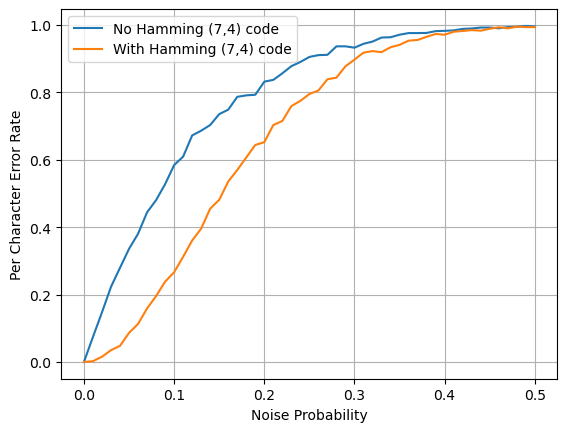
\includegraphics[scale=0.5]{q20.png}
  \caption{Per character error rate as a function of the noise probability}
  \label{fig:q20}
\end{figure}

The "No Hamming (7,4) code" case's high damping curve shows that the error rate rises rapidly as the noise probability rises. This makes sense because every bit flip brought on by noise results in a mistake in the final text if there is no error correction.\\

On the other hand, the sigmoid curve for the "With Hamming (7,4) code" case shows that, at least up to a certain point, the error rate increases more slowly with the noise probability. This is possible because some of the bit flips brought on by the noise can be corrected by the Hamming (7,4) algorithm. The Hamming (7,4) code can only correct one error every 7-bit chunk, hence it loses effectiveness as the noise probability rises. Because of this, the curve gradually begins to rise more quickly, giving rise to the sigmoid function's distinctive S form.

\subsection{Question 21 : } 

To reduce the probability of errors and/or to improve the efficiency of communication, an idea could be the following: First step, compress the text using a data compression algorithm such as Huffman coding, on-line Lempel-Ziv coding or LZ77 coding. Then, second step, encode the binary text signal using Hamming (7,4).

\begin{figure}[H]
  \centering
  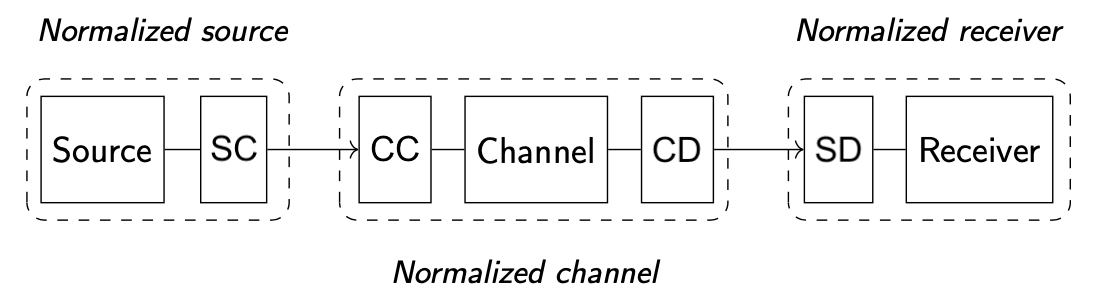
\includegraphics[scale=0.5]{q21.png}
  \caption{Normalized source-channel-receiver scheme}
  \label{fig:q20}
\end{figure}

List of acronyms:
\begin{itemize}
    \item \textbf{SC:} Source Coding
    \item \textbf{CC:} Chanel Coding
    \item \textbf{CD:} Chanel Decoding
    \item \textbf{SD:} Source Decoding
\end{itemize}

The first step would correspond to Source Coding (\textbf{SC}) and reduce the possibilities of errors. The second step would correspond to Chanel Coding (\textbf{CC}) and use the redundant bits to detect and correct any single-bit errors.\\

Source coding aims at making the source messages appear shorter and purely random by deleting redundant information from them. The goal of channel coding, on the other hand, is to provide redundancy to the message so that it can be decoded despite the uncertainty brought on by the channel noise.



\end{document}
